%% infotel.tex 1.4   2016-09-15    Infotel latex template
%------------------------------------------------------------------
% Filename: infotel_template.tex
%
% This file is intended as a template for typesetting articles for the
%
%                        Journal of Spatial Information Science.
%
% Please edit this template to generate your own formatted manuscripts




%%% * All titles and sections lower case *EXCEPT short title  [ ]
%%% * Remove author postal addresses, only have geographic places and institutions [ ] 
%%% * Consistent use of Section, Figure, Table (capitalized and in full) [ ]
%%% * 10 keywords (and all lower case) [ ]
%%% * Remove all avoidable footnotes [ ]
%%% * Use double quotation marks (``'' not "" or `') [ ]
%%% * Punctuation inside quotations [ ]
%%% * E.g. and i.e. followed by comma [ ]
%%% * cf. followed by tilde [ ]
%%% * Itemize and enumerate correctly punctuated [e.g., "1. x, 2. y, and 3. x." ]
%%% * And/or lists using American English punctuation (e.g., "x, y, and z") [ ] 
%%% * Bibliography (e.g., en-dashes for number ranges, consistent "Proc.~" for Proceedings of..., etc.) []
%%% * Acknowledgment style use section* [ ] 
%%% * et al. no italics, but with dot  [ ] 
%%% * All captions end with full stop  [ ] 
%%% * Table captions under, not over table  [ ]
%%% * Adjust urls with burlalt [ ] 
%%% * Check correct use of hyphens, emdashes, endashes  [ ]
%%% * Perform spell check  [ ] 


%%% Check DOI, page numbers on article and web site. [ ]
%%% Update web site with final title, abstract, keywords. [ ] 
%%% Build with distiller for DOI links. [ ]


\documentclass{infotel}
\usepackage{hyperref}
\hypersetup{
	colorlinks=false,
	citecolor=Violet,
	linkcolor=Red,
	urlcolor=Blue}
\usepackage[hyphenbreaks]{breakurl}
\usepackage{booktabs}
\usepackage{stmaryrd}
\usepackage[T1]{fontenc}
\usepackage{cite}
\usepackage{hyperref}
\hypersetup{colorlinks,linkcolor={blue},citecolor={blue},urlcolor={red}}  

% Suggested packages for algorithm formatting
\usepackage{algorithm}
%\usepackage{algorithmic}
\usepackage{algpseudocode}


\usepackage[table]{xcolor}
\usepackage{amssymb,amsmath}


\usepackage{url}
\usepackage{multirow}
\usepackage{cite}
\usepackage{amsmath,amssymb,amsfonts}
\usepackage{graphicx}
\usepackage{textcomp}
\usepackage{xcolor}

\usepackage{tikz}
\usetikzlibrary{positioning, shapes, arrows}


%\setcounter{page}{412}
\renewcommand{\topfraction}{0.9} 
\renewcommand{\textfraction}{0.1}

% Page setup and overhangs
\sloppy
\widowpenalty=10000
\clubpenalty=10000
\hyphenpenalty=75

% Article details for accepted manuscripts will be added by editorial staff
% Omit year if article in press
% Omit number if article under review
\infoteldetails{%
   volume=xx, number=x, month=Month, year=xxxx, firstpage=1, lastpage=10, 
  doi={\href{https://ejournal.ittelkom-pwt.ac.id/index.php/infotel}{10.xxxxx/infotel.vxxix.xxx}},
   received={Month xx, xxxx}, 
   %returned={February 25, 2016},
   revised={Month xx, xxxx},
   accepted={Month xx, xxxx}, }

\newcommand{\mydoi}[1]{\href{http://dx.doi.org/#1}{doi:\protect\detokenize{#1}}}

%\renewcommand{\UrlLeft}{http:\sslash}
%\DeclareUrlCommand\myurl{\def\UrlLeft{}\def\UrlRight{}%
%\urlstyle{tt}}

\urlstyle{rm}
\makeatletter
% Inspired by http://anti.teamidiot.de/nei/2009/09/latex_url_slash_spacingkerning/
% but slightly less kern and shorter underscore
\let\UrlSpecialsOld\UrlSpecials
\def\UrlSpecials{\UrlSpecialsOld\do\/{\Url@slash}\do\_{\Url@underscore}}%
\def\Url@slash{\@ifnextchar/{\kern-.11em\mathchar47\kern-.2em}%
    {\kern-.0em\mathchar47\kern-.08em\penalty\UrlBigBreakPenalty}}
\def\Url@underscore{\nfss@text{\leavevmode \kern.06em\vbox{\hrule\@width.3em}}}
\makeatother

\hypersetup{
colorlinks=true,
linkcolor=black,
citecolor=black,
urlcolor=black
} 

% Add the running author and running title information
\runningauthor{\begin{minipage}{.9\textwidth}\centering Yohannis \textit{et al.}\end{minipage}}
\runningtitle{Towards an IT Framework for Remote Work: an Analysis of Employee Perceptions}

% Document begins
\begin{document}
\setcounter{page}{1}


% Insert your own title
\title{Towards an IT Framework for Remote Work: an Analysis of Employee Perceptions}

% Insert your manuscipts authors, affiliations, and addresses
\author{Alfa Yohannis\textsuperscript{1,*}, Alexander Waworuntu\textsuperscript{2},}
\author{Master Edison Siregar\textsuperscript{3}}
\affil{\textsuperscript{1,2}Informatics Department, Universitas Pradita, Tangerang, Indonesia\\
\textsuperscript{2}Informatics Department, Universitas Multimedia Nusantara, Tangerang, Indonesia}
\affil{*Corresponding email: alfa.ryano@gmail.com}

\maketitle

% Add 5-10 keywords for every submission
\keywords{remote work implementation, employee perceptions, information technology framework, digital work environment, qualitative analysis}

% Add a short abstract of 150-250 words
\begin{abstract}
	This paper presents a qualitative study conducted to identify key components for an IT framework to support the implementation of remote work in Indonesia. The study focuses on employees’ experiences and perceptions during the transition from traditional office-based environments to remote work settings, particularly in response to shifting work norms. It investigates four main aspects: the perceived advantages and disadvantages of remote work, the technological requirements, and the ethical considerations that arise in distributed work arrangements. Data were gathered through an online questionnaire distributed across various sectors, resulting in 97 valid responses. The responses were analysed using qualitative thematic analysis to uncover patterns and common themes. The analysis revealed that employees view flexibility, time efficiency, and reduced commuting expenses as major benefits of remote work. Conversely, communication difficulties, work-life imbalance, and technical constraints were noted as the most significant drawbacks. Furthermore, participants expressed specific expectations for supportive digital tools, robust infrastructure, and ethical standards concerning privacy and fairness. Drawing from these findings, the study identifies six candidate components essential for an IT framework aimed at facilitating effective and sustainable remote work practices. The anonymised dataset has been made publicly available to encourage further research and practical development in the Indonesian remote work context.
\end{abstract}

\section{Introduction}

The COVID-19 pandemic has significantly transformed how employees and organisations conduct work. Many companies shifted from office-based to remote work arrangements to maintain business continuity and employee safety. This transition introduced both benefits and challenges, especially in regions where remote work culture and digital infrastructure were underdeveloped. In Indonesia, the shift highlighted various factors affecting employee productivity, communication, well-being, and ethical considerations.

Although several studies have examined remote work globally, limited research has focused on the Indonesian context, particularly from employees across different industries. Understanding perceived advantages, disadvantages, technological needs, and ethical aspects is essential for organisations aiming to improve remote work policies.

This study addresses this gap by collecting and analysing qualitative data on employees' perceptions of remote and office-based work in Indonesia. The data, gathered through an online survey, provides insights into work preferences, technology use, and ethical concerns. Based on the analysis, the study proposes an IT framework to support remote work implementation. The key contributions are: (1) providing a qualitative dataset on remote and office-based work perceptions in Indonesia; (2) identifying perceived benefits and challenges of different work arrangements; (3) capturing expectations regarding supporting technologies and ; and (4) proposing an IT framework for remote work practices.


\section{Related Work}

Recent studies have examined the transformation of work arrangements, particularly remote and hybrid models, following the COVID-19 pandemic. Yang et al.~\cite{yang2022effects} found that remote work increased flexibility but reduced synchronous communication and cross-team collaboration. Newbold et al.~\cite{Newbold2022NewNormals} proposed a framework for organisational responses to remote work, emphasising socio-technical adjustments.

Münch et al.~\cite{munch2022capabilities} highlighted the role of digital infrastructure in enabling remote service delivery. Leonardi et al.~\cite{Leonardi2024RemoteWork} analysed how remote work reshapes organisational structures and employee autonomy, while Raj et al.~\cite{Raj2023Remote} reported positive correlations between remote work and firm performance, supported by digital infrastructure and managerial readiness.

Keppler and Leonardi~\cite{Keppler2023RelationalConfidence} explored how digital tools foster relational confidence in remote environments. Smite et al.~\cite{Smite2023WFHFlexibility} emphasised the need for flexible post-pandemic work policies, and Fan and Moen~\cite{Fan2023SubjectiveWellbeing} linked remote work with higher well-being levels. Lauring and Jonasson~\cite{Lauring2024Hybrid} critically reviewed hybrid work models, addressing terminology and cultural impacts. Choudhury et al.~\cite{Choudhury2024Hybrid} found that hybrid work supports productivity and employee satisfaction.

While these studies offer valuable insights into remote and hybrid work, most focus on Western contexts and organisational-level analysis. They often overlook socio-cultural conditions in emerging economies and employee-level perceptions. This study addresses these gaps by adopting an inductive qualitative approach to explore employees’ views on remote and office-based work in Indonesia. It contributes to the literature by providing context-specific evidence from an underrepresented workforce and proposing an IT framework grounded in employee-driven insights, offering practical guidance for remote work implementation in developing countries.



\section{Methodology}
\label{sec:methodology}

Data for this research were collected through an online survey\footnote{The questionnaire is available at \url{https://forms.gle/phfgBDmFPEVUU95R8}
} conducted between February and May 2023 via Google Forms. The questionnaire aimed to capture employees' perceptions of remote and office-based work in Indonesia, focusing on advantages, disadvantages, ethical considerations, and technology use. Participants were informed that their data would be used solely for research and could withdraw at any time.

The survey was distributed across various industries using social media platforms (Facebook, LinkedIn, Instagram), messaging apps (WhatsApp, Signal), and direct group chats. Respondents were based in Indonesian cities, including Jakarta, Tangerang, Depok, Bogor, and Bekasi. The responses were compiled into a CSV file, containing data primarily in Indonesian, with partial English translations. The dataset was created to reflect employees' views on remote and office-based work.

A qualitative approach was used to analyse the data, applying inductive thematic analysis \cite{hamilton2019qualitative,kumar2018qualitative}. Responses were categorised into thematic groups and arranged by frequency \cite{seixas2018qualitative,turale2020brief}, providing insights into employee perspectives. The questionnaire also collected demographic and job-related information, including gender, age, industry, job role, responsibilities, and work arrangement preferences. Open-ended questions explored perceived benefits and drawbacks of working from home (WFH), office (WFO), and anywhere (WFA), as well as technologies used and ethical considerations. Detailed descriptions of these variables are provided in Table~\ref{Data Explanation}.


\renewcommand{\arraystretch}{1.3}
\begin{table*}[ht]
	\centering
	\caption{Description of Data Fields}
	\label{Data Explanation}
	\begin{tabular}{p{0.02\textwidth} p{0.16\textwidth} p{0.72\textwidth}}
		\hline
		\textbf{No} & \textbf{Field} & \textbf{Description} \\ 
		\hline
		\textbf{1} & Gender & Information about the gender of the respondents. \\
		\textbf{2} & Age & Age range of the respondents. \\
		\textbf{3} & Industry & Information on the respondents' current workplace or industry. \\
		\textbf{4} & Job Role & Respondents' current position or role at their respective workplaces. \\
		\textbf{5} & Job Task and Responsibility & Descriptions of the respondents' daily job tasks, duties, or responsibilities related to their respective roles. \\
		\textbf{6} & Advantages of WFH & Perceived benefits or positive aspects of working from home (WFH) related to the respondents' jobs. \\
		\textbf{7} & Disadvantages of WFH & Perceived drawbacks or negative aspects of working from home (WFH) related to the respondents' jobs. \\
		\textbf{8} & Advantages of WFO & Perceived benefits or positive aspects of working from the office (WFO) related to the respondents' jobs. \\
		\textbf{9} & Disadvantages of WFO & Perceived drawbacks or negative aspects of working from the office (WFO) related to the respondents' jobs. \\
		\textbf{10} & Advantages of WFA & Perceived benefits or positive aspects of implementing Work From Anywhere (WFA) related to the respondents' jobs. \\
		\textbf{11} & Disadvantages of WFA & Perceived drawbacks or negative aspects of implementing Work From Anywhere (WFA) related to the respondents' jobs. \\
		\textbf{12} & Technology Used in Remote Work & Technologies or applications used by the respondents during WFH or WFA to support their work. \\
		\textbf{13} & Expected Technology in Remote Work & Technologies or applications that the respondents expect to support their work during remote working. \\
		\textbf{14} & Mindset in Remote Work & Collection of mindsets, ethics, norms, and expected behaviours when engaging in remote work. \\
		\textbf{15} & Feasibility of Remote Work in Indonesia & Respondents' perceptions of the challenges and feasibility of implementing remote work in Indonesia. \\
		\hline
	\end{tabular}
\end{table*}





\section{Results and Discussion}
\label{sec:results}

This section presents the results based on the online questionnaire. The discussion highlights key themes from the qualitative analysis, supported by relevant data. A total of 97 responses were collected, and the dataset has been made publicly available on Zenodo at
\url{https://doi.org/10.5281/zenodo.13741856}
~\cite{yohannis2024wfo}.


\subsection{Respondent Industry Profile}
\label{sec:respondent-industry}

Respondents were drawn from various industries to capture diverse perspectives on remote and office-based work. Table~\ref{Respondent Industry} presents the distribution by industry. Most respondents work in education (29 participants), followed by IT (19 participants), both associated with knowledge-based work supporting flexible arrangements. Other sectors include government institutions and consulting services (7 each), clean water supply and property/real estate (6 each), finance (5), and health (3). Additionally, 18 respondents were classified as \textit{Others}. This varied industry profile provides insights into the feasibility and challenges of remote and office-based work across different sectors.

\renewcommand{\arraystretch}{1.3}
\begin{table*}[ht]
	\centering
	\caption{Number of Respondents per Industry}
	\label{Respondent Industry}
	\begin{tabular}{p{.05\textwidth} p{.7\textwidth} r}
		\hline
		\textbf{No.} & \textbf{Industry} & \textbf{Count} \\ 
		\hline
		\textbf{1} & Education (Edu) & 29 \\ 
		\textbf{2} & Information Technology (IT) & 19 \\ 
		\textbf{3} & Government (Gov) & 7 \\ 
		\textbf{4} & Consulting (Cons) & 7 \\ 
		\textbf{5} & Clean Water Supply (CWS) & 6 \\ 
		\textbf{6} & Property/Real Estate (Property) & 6 \\ 
		\textbf{7} & Finance (Fin) & 5 \\ 
		\textbf{8} & Health (Health) & 3 \\ 
		\textbf{9} & Others (Other) & 18 \\ 
		\hline
	\end{tabular}
\end{table*}


\subsection{Perceived Advantages of Working from Home}
\label{sec:advantage-wfh}

The questionnaire included an open-ended question on the advantages of working from home (WFH). Responses were categorised into key themes, as shown in Table~\ref{Advantage of WFH}. The most cited advantage is \textit{time flexibility and efficiency} (76 mentions), reflecting respondents' appreciation of managing their working hours freely. The second is the absence of commuting (38 mentions), consistent with prior studies on remote work benefits. Other advantages include cost savings, particularly on transportation (30 mentions), increased productivity and the ability to perform other tasks (28 mentions), improved well-being (22 mentions), and more time with family (17 mentions). These findings suggest that WFH advantages centre on flexibility, efficiency, and well-being, aligning with existing literature.

\begin{table*}[ht]
	\centering
	\caption{Advantages of WFH}
	\label{Advantage of WFH}
	\begin{tabular}{p{.05\textwidth} p{.7\textwidth} r}
		\hline
		\textbf{No.} & \textbf{The Themes of WFH Advantages} & \textbf{Count} \\ 
		\hline
		\textbf{1} & Time flexibility/Time efficiency (FlexEff) & 76 \\ 
		\textbf{2} & No need for commuting/travelling (NoCom) & 38 \\ 
		\textbf{3} & Cost-saving/Transportation expenses (Cost) & 30 \\ 
		\textbf{4} & Increased productivity/Ability to do other tasks (Prod) & 28 \\ 
		\textbf{5} & Well-Being (Well) & 22 \\ 
		\textbf{6} & More time for family (Fam) & 17 \\ 
		\hline
	\end{tabular}
\end{table*}

\subsection{Perceived Disadvantages of Working from Home}
\label{sec:disadvantage-wfh}

The questionnaire included an open-ended question on the disadvantages of working from home (WFH). Responses were categorised into thematic groups, as summarised in Table~\ref{Disadvantages of WFH}. The most reported disadvantage is \textit{difficulty in time and task management} (45 mentions), indicating challenges in organising work hours. The second is \textit{communication difficulties} (39 mentions), reflecting limitations of remote communication tools. Additionally, 38 respondents noted \textit{difficulty maintaining work-life balance}, while 33 mentioned \textit{difficulty in building professional relationships}. Technical issues were reported by 27 respondents, including internet and hardware problems. A further 18 cited \textit{lack of motivation and self-discipline}, and 9 highlighted negative impacts on \textit{mental or physical well-being}. These findings suggest that WFH flexibility is often accompanied by organisational, social, and technical challenges affecting productivity and well-being.

\renewcommand{\arraystretch}{1.3}
\begin{table}
	\centering
	\caption{Disadvantages of WFH}
	\label{Disadvantages of WFH}
	\begin{tabular}{p{.05\textwidth} p{.7\textwidth} r}
		\hline
		\textbf{No.} & \textbf{The Themes of WFH Disadvantages} & \textbf{Count} \\ 
		\hline
		\textbf{1} & Difficulty in time management and task management (Manage) & 45 \\ 
		\textbf{2} & Difficulty in Communication (Com) & 39 \\ 
		\textbf{3} & Difficulty in maintaining work-life balance (Balance) & 38 \\ 
		\textbf{4} & Difficulty in building professional relationships (Relation) & 33 \\ 
		\textbf{5} & Technical challenges and technology issues (Issue) & 27 \\ 
		\textbf{6} & Lack of motivation and self-discipline (Mov) & 18 \\ 
		\textbf{7} & Mental or physical well-being (Well) & 9 \\ 
		\hline
	\end{tabular}
\end{table}



\subsection{Perceived Advantages of Working from the Office}
\label{sec:advantage-wfo}

The questionnaire explored respondents' perceptions of the advantages of working from the office (WFO). Responses were categorised into key themes, as shown in Table~\ref{Advantage of WFO}. The most mentioned advantage is \textit{effective communication and collaboration} (62 mentions), highlighting the value of face-to-face interaction for clearer, more productive communication. The second is \textit{strong social interaction and work relationships} (33 mentions), reflecting the office's role in fostering networks and social bonds. Additionally, 42 respondents noted that WFO supports \textit{increased focus and productivity}, suggesting the structured office environment helps employees concentrate. These findings show that, despite the flexibility of remote work, many employees value the office for communication, collaboration, and social engagement.



\renewcommand{\arraystretch}{1.3}
\begin{table}
	\centering
	\caption{Advantages of WFO}
	\label{Advantage of WFO}
	\begin{tabular}{p{.05\textwidth} p{.7\textwidth} r}
		\hline
		\textbf{No.} & \textbf{The Themes of WFO Advantages} & \textbf{Count} \\ 
		\hline
		\textbf{1} & Effective communication and collaboration (Effect) & 62 \\ 
		\textbf{2} & Strong social interaction and work relationships (Relation) & 33 \\ 
		\textbf{3} & Increased focus and productivity (Prod) & 42 \\ 
		\hline
	\end{tabular}
\end{table}


\subsection{Perceived Disadvantages of Working from the Office}
\label{sec:disadvantage-wfo}

The questionnaire also explored the perceived disadvantages of working from the office (WFO) through an open-ended question. Responses were categorised into thematic groups, as shown in Table~\ref{Disadvantages of WFO}. The most mentioned disadvantage is \textit{long and tiring commuting time} (56 mentions), highlighting the burden of commuting on well-being and productivity. The second is \textit{lack of flexibility in work hours} (37 mentions), reflecting concerns about rigid schedules and limited work-life balance. Additionally, 27 respondents noted \textit{high transportation costs}, while 14 mentioned other issues, including workplace distractions and reduced autonomy. These findings suggest that WFO disadvantages mainly involve time, cost, and flexibility constraints, contrasting with remote work benefits.

\renewcommand{\arraystretch}{1.3}
\begin{table}
	\centering
	\caption{Disadvantages of WFO}
	\label{Disadvantages of WFO}
	\begin{tabular}{p{.05\textwidth} p{.7\textwidth} r}
		\hline
		\textbf{No.} & \textbf{The Themes of WFO Disadvantages} & \textbf{Count} \\ 
		\hline
		\textbf{1} & Long and tiring commuting time & 56 \\ 
		\textbf{2} & Lack of flexibility in work hours & 37 \\ 
		\textbf{3} & High transportation costs & 27 \\ 
		\textbf{4} & Other & 14 \\ 
		\hline
	\end{tabular}
\end{table}



\subsection{Perceived Advantages of Working from Anywhere}
\label{sec:advantage-wfa}

The questionnaire explored respondents' perceptions of the advantages of working from anywhere (WFA). Responses were categorised into thematic groups, as shown in Table~\ref{Advantages of WFA}. The most mentioned advantage is the \textit{influence of a work environment} (61 mentions), reflecting appreciation for the ability to choose or adjust the workspace to improve comfort, motivation, and productivity. The second is \textit{flexible working hours} (55 mentions), showing the value of temporal flexibility. Additionally, 7 respondents noted \textit{cost savings on transportation}, similar to WFH advantages. These findings suggest that WFA offers benefits related to environmental flexibility, time autonomy, and reduced commuting costs.


\renewcommand{\arraystretch}{1.3}
\begin{table}
	\centering
	\caption{Advantages of WFA}
	\label{Advantages of WFA}
	\begin{tabular}{p{.05\textwidth} p{.7\textwidth} r}
		\hline
		\textbf{No.} & \textbf{The Themes of WFA Advantages} & \textbf{Count} \\ 
		\hline
		\textbf{1} & Influence of a work environment (Env) & 61 \\ 
		\textbf{2} & More flexible working hours (Flex) & 55 \\ 
		\textbf{3} & Cost savings on transportation (Cost) & 7 \\ 
		\hline
	\end{tabular}
\end{table}



\subsection{Perceived Disadvantages of Working from Anywhere}
\label{sec:disadvantage-wfa}

The questionnaire included an open-ended question on the disadvantages of working from anywhere (WFA). Responses were categorised into thematic groups, as shown in Table~\ref{Disadvantages of WFA}. The most frequently mentioned disadvantage is \textit{difficulties in coordination and communication} (27 mentions), reflecting challenges in maintaining effective interaction across locations. The second issue is \textit{limitations of infrastructure and technology} (26 mentions), related to internet access, devices, and software. Additionally, 5 respondents noted \textit{difficulties in social interaction and togetherness}. Another 35 respondents mentioned various concerns, including maintaining discipline, distractions, and uncertainty about company policies. These findings suggest that WFA, despite its flexibility, introduces challenges in communication, infrastructure, and social engagement, potentially affecting productivity and well-being.

\renewcommand{\arraystretch}{1.3}
\begin{table}
	\centering
	\caption{Disadvantages of WFA}
	\label{Disadvantages of WFA}
	\begin{tabular}{p{.05\textwidth} p{.7\textwidth} r}
		\hline
		\textbf{No.} & \textbf{The Themes of WFA Disadvantages} & \textbf{Count} \\ 
		\hline
		\textbf{1} & Difficulties in Coordination and Communication (Com) & 27 \\ 
		\textbf{2} & Limitation of Infrastructure and Technology (Lim) & 26 \\ 
		\textbf{3} & Difficulties in Social Interaction and Togetherness (Soc) & 5 \\ 
		\textbf{4} & Other (Other) & 35 \\ 
		\hline
	\end{tabular}
\end{table}


\subsection{Applications Used for Remote Work}
\label{sec:used-applications}

The questionnaire also gathered information on the applications and platforms used to support remote work, aiming to identify key tools for communication, collaboration, and task management. Table~\ref{Used Application for Remote Work} shows the categories, specific products, and frequency of mentions. The most mentioned category is \textit{Office Suite / Workspace} (176 mentions), including Microsoft Office 365 (OneDrive, Excel, Word, PowerPoint, SharePoint) and Google Workspace (Docs, Sheets, Drive, Gmail, Calendar, Classroom), essential for document creation and administration. The second category is \textit{Online Meeting and Video Conference Platforms} (148 mentions), covering Zoom, Microsoft Teams, Google Meet, Skype, and Webex. Another 84 mentions were recorded under \textit{Other Software and Platforms}, including project management tools (Trello, Asana), creative software (Adobe Creative Cloud, Canva), collaboration platforms (Miro, Padlet), development tools (GitLab, GitHub), and productivity tools. Lastly, 32 mentions were recorded under \textit{Other Communication Applications}, such as WhatsApp, Telegram, Signal, LINE, and Facebook Messenger for informal communication. These findings highlight the variety of digital tools used and the critical role of digital infrastructure in enabling remote work.

\renewcommand{\arraystretch}{1.3}
\begin{table*}
	\centering
	\caption{Used Application for Remote Work}
	\label{Used Application for Remote Work}
	\begin{tabular}{p{0.22\textwidth} p{0.6\textwidth} r}
		\hline
		\textbf{Category} & \textbf{Product} & \textbf{Count} \\ 
		\hline
		\textbf{Office Suite / Workspace (Office)} & OneDrive, Excel, MS Word, PowerPoint, SharePoint, Office 365, Google Docs, Google Sheets, Google Drive, Gmail, Google Calendar, Google Slides, Google Jamboard, Google Forms, Google Sites, Google Classroom & 176 \\ 
		\textbf{Application / Platform for Online Meeting / Video Conference (Meet)} & Zoom, Microsoft Teams, Google Meet, Skype, Webex, GoToMeeting, Discord, Jitsi, Around & 148 \\ 
		\textbf{Other Software / Platform (Other)} & Adobe Creative Cloud, Trello, Asana, Monday.com, Quizziz, Jira, Miro, Padlet, Canva, Capcut, VN editing, ClickUp, Qase, GitLab, GitHub, Bitbucket, Moodle, Prezi, Mentimeter, Kahoot, Standup.ly, SAP, TeamViewer, Anydesk, Fortinet client, Global Protect, Jenkins, Greatday, HRIS, Teramind, Virtual Lab, Visual Studio, Microsoft Visio, WPS Office, PDF, Power BI, MURAL, Notion, Grammarly, QuillBot, VS Code, Figma, AWS, Adobe Sign, VPN, STS & 84 \\ 
		\textbf{Other Communication Apps (Com)} & WhatsApp, Telegram, Signal, LINE, Facebook Messenger, Outlook, Slack & 32 \\ 
		\hline
	\end{tabular}
\end{table*}



\subsection{Desired Applications and Technologies for Remote Work}
\label{sec:desired-apps}

The questionnaire included an open-ended question on applications and technologies that could improve remote work. Responses were categorised by type and purpose, as shown in Table~\ref{tab:required_apps_for_remote_work}. The most mentioned category is \textit{Other applications and software} (42 mentions), covering Microsoft Office, Google applications, online attendance systems, signal stabilisers, and productivity tools. The second category is \textit{Communication and Collaboration Applications} (30 mentions), highlighting the need for reliable platforms like Zoom, Google Meet, Microsoft Teams, and AI-based tools such as ChatGPT. The third category is \textit{Internet and IT Infrastructure} (28 mentions), emphasising the need for stable, high-speed, and portable internet, followed by \textit{Technology and Devices} (26 mentions), including laptops, smartphones, tablets, and built-in connectivity. Respondents also mentioned \textit{Supporting Applications for Work and Productivity} (19 mentions), covering time management, monitoring, and evaluation systems, as well as advanced technologies like \textit{AI, IoT, and Machine Learning} (10 mentions). A smaller group (7 mentions) highlighted immersive technologies like \textit{VR and 3D virtual meetings}, while 9 mentions were recorded under \textit{Other Systems}, including Mini World platforms, software upgrades, and enhanced learning media. These findings indicate that employees expect a broad range of technologies beyond communication tools to support remote work.

\renewcommand{\arraystretch}{1.3}
\begin{table*}[ht]
	\centering
	\caption{Desired applications to have for remote work.}
	\label{tab:required_apps_for_remote_work}
	\begin{tabular}{p{0.25\textwidth} p{0.58\textwidth} r}
		\hline
		\textbf{Category} & \textbf{Item} & \textbf{Count} \\ 
		\hline
		\textbf{Communication and collaboration apps or software (Com)} & Online Meeting Applications (Zoom, Google Meet, etc.), Interaction Integration, ChatGPT, Collaboration Applications (WhatsApp, Telegram, etc.), Microsoft Teams, Discord & 30 \\ 
		\textbf{Internet and IT infrastructure (Int)} & Stable and Fast Internet, Broadband, Portable Internet Connection, Internet that can be used anywhere, High-Speed Internet & 28 \\ 
		\textbf{Technology and devices (Dev)} & Laptop, High-Specification Laptops, Smartphone/Cellphone, Tablet/iPad, Signature validation, Office-provided Hardware, Built-in Internet Devices in Laptops & 26 \\ 
		\textbf{Supporting apps for work and productivity (Sup)} & Integrated System, Technology for Calculating Work Progress, Time Management, Kanban Board, Result-Based System & 19 \\ 
		\textbf{AI, IoT, and Machine Learning (AI)} & AI, IoT, Machine Learning & 10 \\ 
		\textbf{VR and 3D Virtual Meeting (VR)} & VR, 3D Virtual Meeting & 7 \\ 
		\textbf{Other applications and software (Oapp)} & Microsoft Office (Excel, Word, etc.), Google Software, Free Software, Online Attendance Software, Presentation Recording Software, Online Exam Monitoring Software, Signal Stabilizer Software, Voice-Based Report Generator Software, Integrated Company Devices, Single Sign-On, Digital Intelligence Assistance, Mobile Monitor Extender & 42 \\ 
		\textbf{Other system (Osys)} & Mini World, 2D to 4D Projector, Software Feature Upgrades, Integrated Administration System, Enhanced MS Teams, Digitalization of Learning Media & 9 \\ 
		\hline
	\end{tabular}
\end{table*}



\subsection{Expected Ethics and Norms for Remote Work}
\label{sec:ethics-remote-work}

The questionnaire included an open-ended question to identify ethics, norms, and behaviours considered essential for remote work. Responses were categorised into four ethical themes, as summarised in Table~\ref{tab:ethics_for_remote_work}. The most frequently mentioned theme is \textit{Work Ethics and Responsibilities} (137 mentions), covering responsibility, discipline, and integrity, with the most cited subgroup being \textit{Timely Contact by Superiors, Managers, and Colleagues} (43 mentions). Other subgroups include responsibility towards work, dress code, independence, orderliness, honesty, ethical trust, and accountability. The second theme is \textit{Communication and Collaboration} (63 mentions), with key subgroups such as the expectation to \textit{Turn on the Camera during Video Calls} (21 mentions) and \textit{Clear and Effective Communication} (20 mentions), along with polite communication, email etiquette, and regular meetings. The third theme, \textit{Efficiency and Productivity} (22 mentions), includes adherence to \textit{Standard Operating Procedures} (12 mentions), meeting efficiency, procedure revision, continuous learning, and screen monitoring. The fourth theme is \textit{Performance Measurement} (20 mentions), mainly related to \textit{Objective-Based Performance Measurement} (19 mentions). These findings suggest that employees expect clear ethical guidelines covering responsibility, communication, productivity, and fair performance evaluation in remote work settings.


\renewcommand{\arraystretch}{1.3}
\begin{table*}[ht]
	\centering
	\caption{Ethics and Norms for Remote Work}
	\label{tab:ethics_for_remote_work}
	\begin{tabular}{p{0.23\textwidth} p{0.55\textwidth} r r}
		\hline
		\textbf{Ethics of Remote Work} & \textbf{Sub Group Ethics of Remote Work} & \textbf{Qty} & \textbf{Total} \\ 
		\hline
		\multirow{8}{=}{Work Ethics and Responsibilities (Resp)}   
		& Timely Contact by Superiors with Employees, Managers, and Colleagues (Time) & 43 & \multirow{8}{*}{137} \\ 
		& Responsibility towards Work (Resp) & 30 & \\ 
		& Dress Code Guidelines (Dress) & 19 & \\ 
		& Independence and Trust (Ind) & 13 & \\ 
		& Orderliness in Attendance Recording and Report Submission (Ord) & 13 & \\ 
		& Honesty and Integrity (Hon) & 10 & \\ 
		& Ethical Trust in the Workplace (Ethical) & 6 & \\ 
		& Trust and Responsibility in Performing Individual Roles (Indiv) & 3 & \\ 
		\hline
		
		\multirow{6}{=}{Communication and Collaboration (Com)}    
		& Turning on the camera during a video call (Cam) & 21 & \multirow{6}{*}{63} \\ 
		& Clear and Effective Communication (Eff) & 20 & \\ 
		& Polite Communication (Polite) & 13 & \\ 
		& The tone of a sentence in an email (Tone) & 5 & \\ 
		& Weekly Meeting to Discuss Work (Meet) & 3 & \\ 
		& Good Communication (Good) & 1 & \\ 
		\hline
		
		\multirow{5}{=}{Efficiency and Productivity (Eff)}    
		& Procedures (SOP) regarding working hours (SOP) & 12 & \multirow{5}{*}{22} \\ 
		& Meeting Efficiency (Eff) & 4 & \\ 
		& Revision of Standard Operating (Rev) & 3 & \\ 
		& Continuous Learning (Learn) & 2 & \\ 
		& Utilization of Screen Monitoring Applications (Screen) & 1 & \\ 
		\hline
		
		\multirow{2}{=}{Performance Measurement (Perf)} 
		& Objective-Based Performance Measurement (Obj) & 19 & \multirow{2}{*}{20} \\ 
		& Performance Assessment Based on Platforms (Plat) & 1 & \\ 
		\hline
	\end{tabular}
\end{table*}


\section{IT Framework Components for Remote Work Implementation}
\label{sec:it-framework}

Based on the findings in Section~\ref{sec:results}, key components for an IT framework to support remote work can be identified. These components are derived from respondents’ perceptions of remote work advantages, disadvantages, ethical considerations, technology use, and feasibility factors, as summarised in Tables~\ref{Advantage of WFH}, \ref{Disadvantages of WFH}, \ref{Advantage of WFO}, \ref{Disadvantages of WFO}, \ref{Advantages of WFA}, \ref{Disadvantages of WFA}, \ref{Used Application for Remote Work}, \ref{tab:required_apps_for_remote_work}, and \ref{tab:ethics_for_remote_work}.

\textbf{Governance and Policy.}
Clear ethical guidelines and measurable performance indicators are necessary (Table~\ref{tab:ethics_for_remote_work}). The framework should include: (1) \textit{Remote Work Guidelines} on conduct, communication, and working hours; (2) \textit{Performance Measurement} through objective evaluation; and (3) \textit{Attendance and Reporting Procedures}. Establishing formal remote work policies and clear key performance indicators is essential for maintaining productivity and ensuring equitable treatment of all employees \cite{Waizenegger2020, Charalampous2019 }.

\textbf{Digital Skills and Awareness.}
Findings indicate challenges in communication, discipline, and technology use (Tables~\ref{Disadvantages of WFH}, \ref{Disadvantages of WFA}). The framework should cover: (1) \textit{Capacity Building} through training; and (2) \textit{Remote Work Mindset Development} programmes. Success in a remote setting requires employees to develop not only digital competencies for new technologies but also stronger self-regulation skills to manage their autonomy and maintain performance \cite{Waizenegger2020, Charalampous2019 }.

\textbf{Employee Well-being and Work-Life Balance.}
Maintaining well-being and balance is a key concern (Tables~\ref{Disadvantages of WFH}, \ref{Disadvantages of WFO}). The framework should include: (1) \textit{Well-being Monitoring} channels; and (2) \textit{Work-Life Balance Policies} encouraging flexibility and limiting working hours. Without formal support mechanisms, remote work can blur the boundaries between professional and personal life, leading to exhaustion and a decline in job satisfaction \cite{Charalampous2019, Oakman2020}.

\textbf{Application Ecosystem.}
Respondents reported using various digital applications to support remote work (Table~\ref{Used Application for Remote Work}). The framework should provide an integrated ecosystem, including: (1) \textit{Communication and Collaboration Tools} like Zoom and Microsoft Teams; (2) \textit{Productivity Applications} for task and project management; (3) \textit{Document and Workspace Systems} such as Office 365 and Google Workspace; and (4) \textit{Advanced Technologies}, including AI-based tools (Table~\ref{tab:required_apps_for_remote_work}). The effective integration of these tools into a cohesive "digital workplace" is a key determinant of organizational success, with emerging AI capabilities offering new avenues for enhancing collaborative efficiency \cite{Waizenegger2020, Vartiainen2020}.


\textbf{Infrastructure Readiness.}
Reliable internet access and adequate hardware are essential for remote work. Respondents highlighted the need for \textit{stable, high-speed internet} and \textit{company-provided devices} (Table~\ref{tab:required_apps_for_remote_work}). The framework should include: (1) \textit{Reliable Internet Access}; (2) \textit{Device Provision} with standardised hardware; and (3) \textit{Security Infrastructure}, such as VPN, single sign-on (SSO), and multi-factor authentication (MFA). Establishing this baseline infrastructure is critical not only for productivity but also for ensuring equitable access across the workforce and mitigating the significant cybersecurity risks inherent in remote operations \cite{Waizenegger2020, Oakman2020}.


\textbf{Support and Troubleshooting Mechanism.}
Technical issues were highlighted by respondents (Tables~\ref{Disadvantages of WFH}, \ref{Disadvantages of WFA}). The framework should offer: (1) \textit{IT Helpdesk and Remote Assistance}; and (2) \textit{Technical Support Procedures}. When technology fails, it can severely constrain remote collaboration, making a structured and responsive IT support system a critical component of any digital transformation towards remote work  \cite{Waizenegger2020, Charalampous2019}.


These components provide a comprehensive IT framework addressing the technical, ethical, and organisational aspects of remote work, aligned with the needs identified in the analysis.


\begin{figure}[ht]
	\centering
	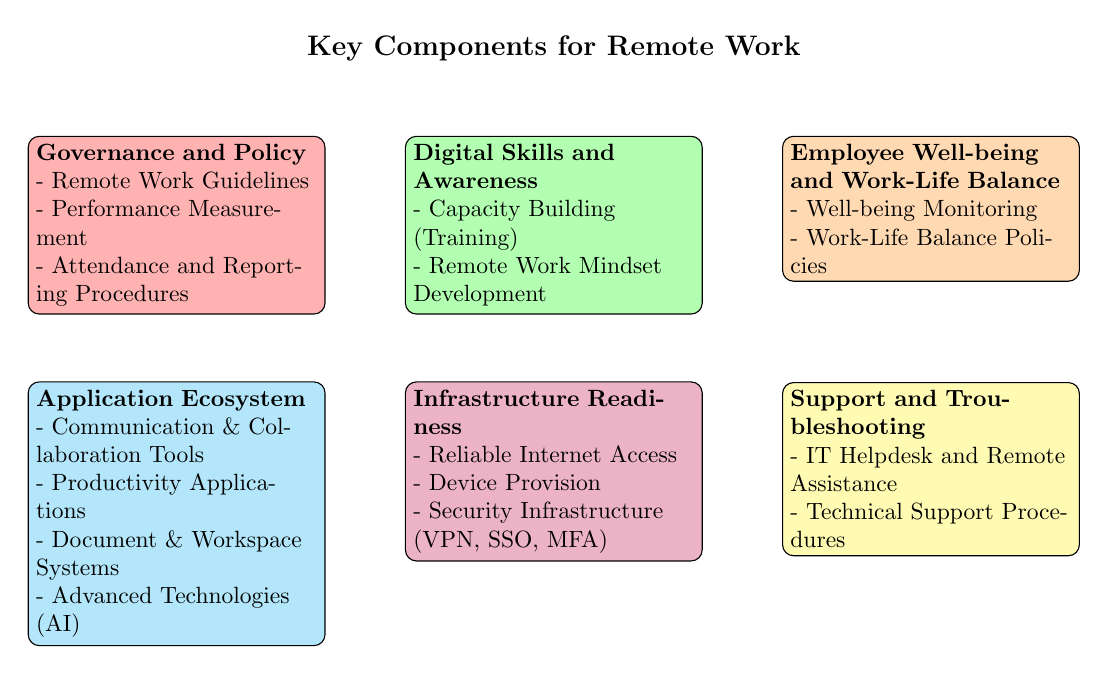
\begin{tikzpicture}[
		scale=0.85, transform shape,
		node distance=10mm and 1mm,
		box/.style={rectangle, draw, rounded corners, text width=4.2cm, align=left, fill=#1!30},
		title/.style={font=\bfseries\large}
		]
		
		% Title at top center
		\node[title] (title) {Key Components for Remote Work};
		
		% First row: three components with subcomponents inside
		\node[box=red, below left=of title, xshift=0.5cm] (gov) {%
			\textbf{Governance and Policy} \\ 
			- Remote Work Guidelines \\
			- Performance Measurement \\
			- Attendance and Reporting Procedures
		};
		
		\node[box=green, below=of title] (skills) {%
			\textbf{Digital Skills and Awareness} \\ 
			- Capacity Building (Training) \\
			- Remote Work Mindset Development
		};
		
		\node[box=orange, below right=of title, xshift=-0.5cm] (wellbeing) {%
			\textbf{Employee Well-being and Work-Life Balance} \\ 
			- Well-being Monitoring \\
			- Work-Life Balance Policies
		};
		
		% Second row: three components with subcomponents inside
		\node[box=cyan, below=1cm of gov] (app) {%
			\textbf{Application Ecosystem} \\ 
			- Communication \& Collaboration Tools \\
			- Productivity Applications \\
			- Document \& Workspace Systems \\
			- Advanced Technologies (AI)
		};
		
		\node[box=purple, below=1cm of skills] (infra) {%
			\textbf{Infrastructure Readiness} \\ 
			- Reliable Internet Access \\
			- Device Provision \\
			- Security Infrastructure (VPN, SSO, MFA)
		};
		
		\node[box=yellow, below=1.5cm of wellbeing] (support) {%
			\textbf{Support and Troubleshooting} \\ 
			- IT Helpdesk and Remote Assistance \\
			- Technical Support Procedures
		};
		
	\end{tikzpicture}
	\caption{Six key components and their subcomponents integrated within each box.}
	\label{fig:key_components_remote_work}
\end{figure}



\begin{figure}[ht]
	\centering
	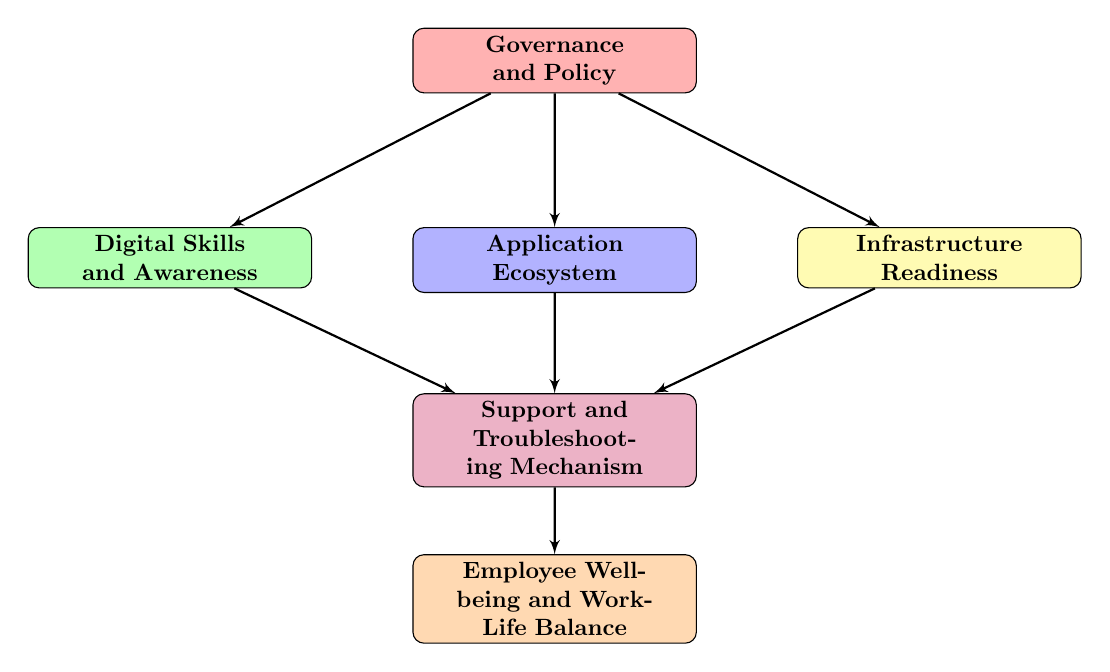
\begin{tikzpicture}[
		scale=0.85, transform shape,
		node distance=10mm and 5mm,
		box/.style={rectangle, draw, rounded corners, text width=4cm, align=center, fill=#1!30},
		line/.style={draw, thick, -latex'}
		]
		
		% Governance (start)
		\node[box=red] (gov) {\textbf{Governance and Policy}};
		
		% Parallel branches
		\node[box=green, below left=of gov, xshift=-1cm, yshift=-1cm] (skills) {\textbf{Digital Skills and Awareness}};
		\node[box=blue, below=of gov, yshift=-1cm] (app) {\textbf{Application Ecosystem}};
		\node[box=yellow, below right=of gov, xshift=1cm, yshift=-1cm] (infra) {\textbf{Infrastructure Readiness}};
		
		% Support below parallel branches
		\node[box=purple, below=1.5cm of app] (support) {\textbf{Support and Troubleshooting Mechanism}};
		
		% Well-being at bottom as continuous
		\node[box=orange, below=of support] (wellbeing) {\textbf{Employee Well-being and Work-Life Balance}};
		
		% Connections
		\path[line] (gov) -- (skills);
		\path[line] (gov) -- (app);
		\path[line] (gov) -- (infra);
		
		\path[line] (skills) -- (support);
		\path[line] (app) -- (support);
		\path[line] (infra) -- (support);
		
		\path[line] (support) -- (wellbeing);
		
	\end{tikzpicture}
	\caption{Sequential and parallelisable components for implementing remote work framework.}
	\label{fig:parallel_components_remote_work}
\end{figure}


\section{Sequential Framework for Remote Work Implementation}

This section discusses the proposed sequential framework to implement effective and sustainable remote work practices, based on the six key components identified from the study. The framework adopts a top-down approach inspired by TOGAF \cite{TheOpenGroup2018}, enterprise architecture best practices \cite{Ross2006}, and IT strategy frameworks \cite{Henderson1993}, ensuring that organisational policies, people readiness, technology, and operational support are addressed systematically.

\textbf{1. Governance and Policy.}  
Governance and Policy serve as the foundation of the framework. It establishes the organisational rules, guidelines, financial considerations, and evaluation mechanisms required to manage remote work effectively. This includes defining Remote Work Guidelines on employee conduct, communication standards, and working hours; Performance Measurement systems to ensure accountability and productivity; Attendance and Reporting Procedures for operational monitoring; and policies to maintain Employee Well-being and Work-Life Balance. Governance and Policy also encompass aligning remote work initiatives with broader business goals and strategies to ensure that remote work supports organisational competitiveness, service delivery, and innovation objectives. Financial aspects such as budgeting for remote work infrastructure, licensing costs for digital applications, employee reimbursements for connectivity or devices, and long-term cost-benefit analyses should be addressed within this component. As the strategic anchor, Governance and Policy must be addressed first before rolling out other operational components to ensure clarity, compliance, alignment with strategic goals, and financial feasibility.

\textbf{2. Digital Skills and Awareness.}  
Once governance structures are established, organisations need to prepare their workforce. Digital Skills and Awareness cover Capacity Building through targeted training programmes to equip employees with essential technical skills, and Remote Work Mindset Development initiatives to foster adaptability, autonomy, and responsible remote work ethics. This component can be developed in parallel with Application Ecosystem planning, ensuring that employees are ready to utilise the tools effectively upon deployment.

\textbf{3. Application Ecosystem.}  
The Application Ecosystem involves providing an integrated suite of digital tools necessary for remote work operations. This includes Communication and Collaboration Tools such as Zoom or Microsoft Teams; Productivity Applications for task and project management; Document and Workspace Systems like Office 365 and Google Workspace; and Advanced Technologies including AI-based tools to enhance efficiency. While deployment depends on infrastructure readiness, planning and configuration can proceed in parallel with Digital Skills development.

\textbf{4. Infrastructure Readiness.}  
A reliable technological foundation is essential for any remote work strategy. Infrastructure Readiness includes ensuring Reliable Internet Access for all staff; Device Provision with standardised and secure hardware; and implementation of Security Infrastructure such as VPNs, Single Sign-On (SSO), and Multi-Factor Authentication (MFA) to protect organisational assets. Device provisioning and network upgrades can commence in parallel with Skills and Application preparation, but Security Infrastructure setup must align with Governance policies defined earlier.

\textbf{5. Support and Troubleshooting Mechanism.}  
To maintain operational continuity, Support and Troubleshooting Mechanisms must be established. This involves setting up an IT Helpdesk for day-to-day assistance, Remote Assistance services for distributed teams, and Technical Support Procedures for efficient issue resolution. This component should be operational before or alongside the final deployment of applications and infrastructure to ensure immediate support during rollout.

\textbf{6. Employee Well-being and Work-Life Balance.}  
Employee Well-being and Work-Life Balance are addressed as a continuous and integrated pillar of the framework. Organisations should implement Well-being Monitoring channels to track employee health and morale, and enforce Work-Life Balance Policies that encourage flexibility while preventing overwork. Although it is discussed last in the sequence, well-being initiatives should be embedded across all stages to ensure sustainable remote work adoption.




\section{Threats to Validity and Limitations}

This study faces several validity threats and limitations. The data were collected through an online questionnaire using convenience sampling, which may introduce sampling bias and limit the representativeness of the respondents, who were primarily recruited via social media and messaging platforms in selected Indonesian cities. The reliance on self-reported perceptions may also be influenced by subjective interpretations and social desirability bias. Additionally, the qualitative analysis focused on frequently mentioned themes, potentially overlooking nuanced insights or minority views. The data collection period in early 2023 may not capture subsequent developments in remote work practices. Furthermore, the findings and proposed IT framework are specific from the Indonesian context and may require adaptation if implemented in other settings. Future studies should consider more diverse samples and longitudinal approaches to capture evolving remote work experiences.

\section{Conclusion and Future Work}

This study analysed employees' perceptions of remote and office-based work in Indonesia, identifying key advantages, disadvantages, and expectations regarding technology use and ethical norms. The findings informed the development of an IT framework to support remote work implementation, covering infrastructure, application ecosystem, governance, digital skills, well-being, technical support, and risk management. Future research should involve a larger, more diverse sample to improve generalisability and consider quantitative or mixed-method approaches to enrich the findings. Further studies may also evaluate the framework's effectiveness in organisational contexts and examine the long-term impact of remote work on employee performance and well-being.

\section*{Acknowledgement}

This research is supported by Universitas Pradita. AI tools were used to assist in improving the grammar and sentence structure of the manuscript prepared by the authors.

\bibliographystyle{infotelacm}
\bibliography{infotelexample}

\end{document}